% ============================================================
% report_skeleton.tex  —  SCHELETRO strutturale
%   Sezioni + figure + tabelle + equazioni, nessun testo narrativo.
%   Usare per discutere la struttura con i colleghi prima di scrivere.
%
% Compilazione: pdflatex -> bibtex -> pdflatex x 2
% ============================================================

\documentclass[11pt, a4paper]{article}

% ── Lingua e font ──────────────────────────────────────────────────────────────
\usepackage[T1]{fontenc}
\usepackage[utf8]{inputenc}
\usepackage[italian]{babel}
\usepackage{lmodern}
\usepackage{microtype}

% ── Layout ─────────────────────────────────────────────────────────────────────
\usepackage{geometry}
\geometry{top=2.8cm, bottom=2.8cm, left=2.8cm, right=2.8cm}
\usepackage{setspace}
\setstretch{1.15}

% ── Matematica ─────────────────────────────────────────────────────────────────
\usepackage{amsmath, amssymb, bm}
\usepackage{mathtools}

% ── Tabelle ────────────────────────────────────────────────────────────────────
\usepackage{booktabs}
\usepackage{array}
\usepackage{multirow}
\usepackage{longtable}
\usepackage{siunitx}
\sisetup{round-mode=places, round-precision=3, detect-weight=true}

% ── Figure ─────────────────────────────────────────────────────────────────────
\usepackage{graphicx}
\graphicspath{{images/}}
\usepackage{caption}
\usepackage{subcaption}
\usepackage{float}

% ── Colori e stile ─────────────────────────────────────────────────────────────
\usepackage{xcolor}
\definecolor{myblue}{HTML}{2C5F8A}
\definecolor{mygray}{HTML}{5A5A5A}
\usepackage{hyperref}
\hypersetup{colorlinks=true, linkcolor=black, citecolor=black, urlcolor=black}

% ── Sezioni ────────────────────────────────────────────────────────────────────
\usepackage{titlesec}
\titleformat{\section}
  {\large\bfseries}{\thesection.}{0.5em}{}
\titleformat{\subsection}
  {\normalsize\bfseries}{\thesubsection.}{0.5em}{}

% ── Intestazioni ───────────────────────────────────────────────────────────────
\usepackage{fancyhdr}
\pagestyle{fancy}
\fancyhf{}
\fancyhead[L]{\small Profili verticali di nutrienti del suolo --- Analisi bayesiana}
\fancyhead[R]{\small\thepage}
\renewcommand{\headrulewidth}{0.3pt}

% ── Bibliografia ───────────────────────────────────────────────────────────────
\usepackage[round, authoryear]{natbib}
\bibliographystyle{apalike}

% ── Comandi matematici custom ──────────────────────────────────────────────────
\newcommand{\Nrm}{\mathcal{N}}
\newcommand{\HN}{\mathcal{N}^{+}}
\newcommand{\E}{\mathbb{E}}
\newcommand{\Var}{\mathrm{Var}}
\newcommand{\SOC}{\mathrm{SOC}}
\renewcommand{\vec}[1]{\bm{#1}}
\newcommand{\CI}[2]{[#1,\;#2]}
\newcommand{\tauA}[1]{\tau_{\alpha,#1}}
\newcommand{\tauB}[1]{\tau_{\beta,#1}}

% ── Placeholder testo ─────────────────────────────────────────────────────────
\newcommand{\todo}[1]{\textcolor{red}{\textit{[#1]}}}

% ── Titolo ─────────────────────────────────────────────────────────────────────
\title{%
  {\Large Analisi gerarchica bayesiana dei}\\[4pt]
  {\huge\bfseries Profili verticali di nutrienti del suolo}\\[4pt]
  {\large\bfseries SOC, N e P in 40 campi agricoli in Tanzania}
}
\author{
  Bortoletto Davide \, Faedo Piero \, Paganelli Gabriele \, Zannini Pietro \\[4pt]
  {\small Statistica Iterazione \,$\cdot$\, Universit\`a degli Studi di Padova, a.a.~2025/26}
}
\date{8 giugno 2026}


% ==============================================================================
\begin{document}
% ── Abstract in inglese (sovrascrive "Sommario" di babel/italian) ──────────────
\renewcommand{\abstractname}{Abstract}
\maketitle
\thispagestyle{empty}

% ── Abstract ──────────────────────────────────────────────────────────────────
\begin{abstract}
\noindent
La distribuzione verticale dei nutrienti del suolo è un indicatore chiave della qualità agronomica, ma i meccanismi che determinano le differenze tra campi nella forma del profilo di profondità restano poco quantificati. In questo lavoro analizziamo i profili verticali di carbonio organico (SOC), azoto totale e fosforo totale in 40 campi agricoli, con misurazioni a fino a sei profondità per campo, per un totale di 220 osservazioni. Sviluppiamo un modello bayesiano gerarchico con pendenza proporzionale che stima esplicitamente come la variabilità inter-campo del profilo verticale cambi con la profondità. I risultati mostrano che i campi con maggiore contenuto medio di SOC presentano profili significativamente più uniformi: la fertilità carboniosa si conserva meglio in profondità. Per l'azoto questo pattern è assente; per il fosforo è presente con evidenza moderata. La selezione predittiva identifica la tessitura fine (contrasto argilla/limo) come principale predittore within-field, mentre le pratiche di gestione risultano essenzialmente non significative dopo aver controllato per la struttura fisica del suolo. A differenza degli approcci standard basati su confronti stratificati per profondità, il modello proposto fornisce stime inferenziali dirette della relazione tra livello medio di campo e forma del profilo verticale, aprendo la strada a una caratterizzazione quantitativa dell'eterogeneità agronomica tra campi.
\end{abstract}

\newpage
\tableofcontents
\newpage


% ==============================================================================
\section{Introduzione}
\label{sec:intro}

\todo{$\sim$1 pagina. Importanza SOC/N/P nell'agricoltura tropicale;
struttura verticale come indicatore di fertilit\`a; domanda di ricerca
(il decadimento con la profondit\`a dipende dal livello medio del campo?);
struttura del paper.}


% ==============================================================================
\section{Dati}
\label{sec:dati}

\subsection{Disegno campionario}

\todo{$J=40$ campi in Tanzania, $N\approx 220$ obs, fino a 6 profondit\`a
per campo (Bottom 10--120\,cm).}

\subsection{Variabili risposta}

\[
  y_r = \log(\text{Perc}_r), \quad r \in \{\SOC, N, P\}.
\]

\subsection{Covariate}

\begin{table}[htbp]
  \centering
  \caption{Statistiche descrittive ($N = 220$ osservazioni, $J = 40$ campi).}
  \label{tab:desc}
  \small
  \begin{tabular}{@{}lrrrrr@{}}
    \toprule
    Variabile & Media & SD & Min & Mediana & Max \\
    \midrule
    SOC (\%)                    & 1.304  & 1.047 & 0.010 & 1.059 & 5.489 \\
    N totale (\%)               & 0.105  & 0.062 & 0.010 & 0.100 & 0.390 \\
    P totale (\%)               & 0.105  & 0.098 & 0.010 & 0.080 & 0.920 \\
    Profondit\`a (cm)           & 43.6   & 17.8  & 20.0  & 40.0  & 80.0  \\
    Texture1 (ILR$_1$)          & $-0.635$ & 0.331 & $-2.040$ & $-0.630$ & 0.458 \\
    Texture2 (ILR$_2$)          & 1.118  & 0.563 & $-0.412$ & 1.139 & 2.572 \\
    Densit\`a app.\ (g/cm$^3$) & 1.36   & 0.35  & 0.62  & 1.28  & 2.06  \\
    pH                          & 5.72   & 0.34  & 4.84  & 5.69  & 6.99  \\
    \midrule
    \multicolumn{6}{@{}l}{\small\textit{Variabili di gestione (between-field, 0/1):}} \\
    \quad OnFarm      & \multicolumn{5}{l}{30/40 campi (75\%)} \\
    \quad Irrigate    & \multicolumn{5}{l}{25/40 campi (62\%)} \\
    \quad Fertilised  & \multicolumn{5}{l}{20/40 campi (50\%)} \\
    \quad N\_Natural  & \multicolumn{5}{l}{5/40 campi (12\%)}  \\
    \bottomrule
  \end{tabular}
\end{table}

ILR (base di Helmert via \texttt{compositions::ilr}):
\[
  T_1 = \sqrt{\tfrac{1}{2}}\,\log\!\left(\frac{\text{Clay}}{\text{Silt}}\right),
  \qquad
  T_2 = \sqrt{\tfrac{2}{3}}\,
        \log\!\left(\frac{\sqrt{\text{Clay}\cdot\text{Silt}}}{\text{Sand}}\right).
\]


\begin{figure}[htbp]
  \centering
  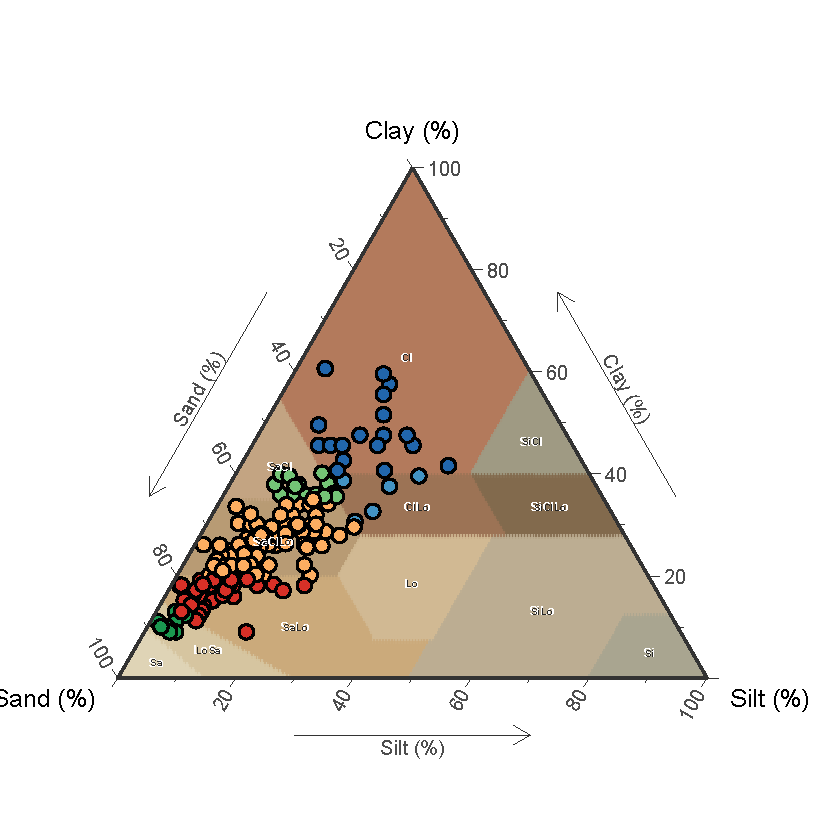
\includegraphics[width=0.55\linewidth]{fig_texture_triangle.pdf}
  \caption{Triangolo USDA delle classi tessiturali per le 220 osservazioni.
    Le classi dominanti sono argilla-limosa (silty clay) e limo-argillosa (clay loam),
    con variabilit\`a sostanziale tra i 40 campi.}
  \label{fig:texture_triangle}
\end{figure}


% ==============================================================================
\section{Analisi esplorativa}
\label{sec:eda}

\subsection{Scelta della forma funzionale}

\subsection{Variabilit\`a tra campi: ICC}

\todo{ICC $\approx 0.72$ per logSOC dal modello nullo lmer; random intercept
necessario e ben identificato.}

\subsection{Profili verticali individuali}
RENDERE VERTICALE e aggiungere P e togliere scritte brutte

\begin{figure}[htbp]
  \centering
  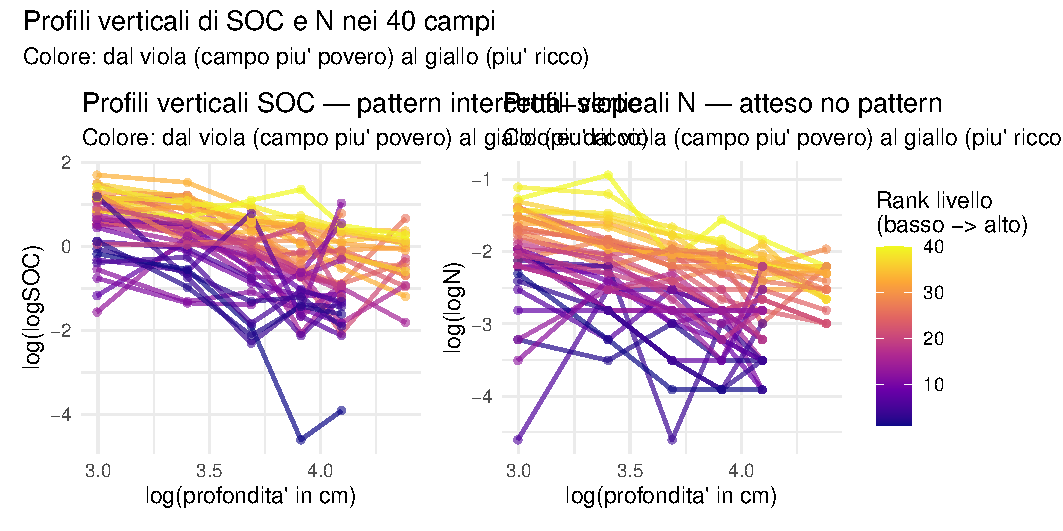
\includegraphics[width=0.8\linewidth]{fig02_spaghetti.pdf}
  \caption{Spaghetti plot dei profili verticali di logSOC (colorati per livello
    medio del campo) e logN (grigio). I campi con SOC elevato mostrano profili
    pi\`u piatti.}
  \label{fig:spaghetti}
\end{figure}

\subsection{Correlazione intercetta--slope: motivazione empirica di M-SP}

\begin{figure}[htbp]
  \centering
  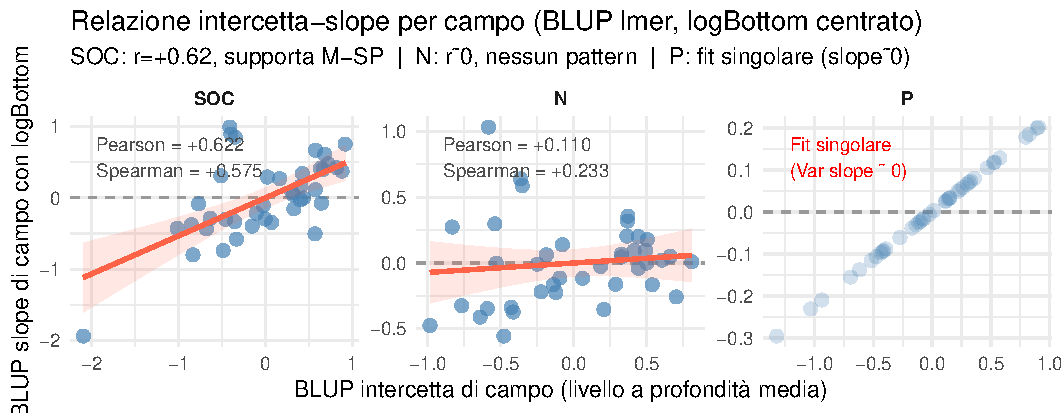
\includegraphics[width=0.8\linewidth]{fig03_scatter.pdf}
  \caption{rimuovibile}
  \label{fig:scatter}
\end{figure}

A parole: correlazione tra slope e intercept

\subsection{Struttura spaziale}

\todo{Moran's I e semivariogramma: nessuna autocorrelazione significativa per
N e P; SOC debole. Conclusione: GP non necessario (confermato da LOO-CV,
Sezione~\ref{subsec:loo4}).}


% ==============================================================================
\section{Modello statistico e inferenza}
\label{sec:modello}

\subsection{Selezione dell'approccio modellistico}

Alla luce delle caratteristiche dei dati e della struttura suggerita dai primi modelli esplorativi, si propone un modello che tiene conto degli effetti fissi delle covariate, specifiche del singolo campo e del singolo carotaggio, oltre ad effetti casuali che catturano la variabilità tra campi sia nel livello medio sia nella rapidità di decadimento delle sostanze lungo il profilo. La struttura gerarchica consente inoltre di modellare congiuntamente le tre risposte (SOC, N e P), permettendo correlazioni tra gli effetti casuali appartenenti allo stesso campo. Si assume invece indipendenza condizionale tra i residui delle tre risposte. L'approccio bayesiano è adottato per favorire il \textit{borrowing of information} tra parametri e garantire maggiore stabilità inferenziale in presenza di un numero elevato di parametri rispetto alla dimensione del campione.

\subsection{Struttura del modello finale}
\label{subsec:msp}

Per ogni risposta $r \in \{1,2,3\}$ (SOC, N e P) e osservazione $i$ nel campo $j$:

\[
  y_{r,ij}
  \sim
  \mathcal{N}\!\bigl(\mu_{r,ij},\sigma_r^2\bigr),
\]

\[
  \mu_{r,ij}
  =
  \alpha_r
  +
  u_{rj}
  +
  v_{rj}\log B_i
  +
  \boldsymbol{\gamma}_r^\top \mathbf{x}_{W,i}
  +
  \boldsymbol{\beta}_r^\top \mathbf{x}_{B,j}.
\]

Gli effetti casuali di campo sono modellati congiuntamente come

\[
  \mathbf b_j
  =
  \bigl(
  u_{1j},v_{1j},
  u_{2j},v_{2j},
  u_{3j},v_{3j}
  \bigr)^\top
  \sim
  \mathcal N_6(\mathbf 0,\Sigma),
\]

con

\[
  \Sigma
  =
  \operatorname{diag}(\boldsymbol{\tau})
  \,
  \Omega
  \,
  \operatorname{diag}(\boldsymbol{\tau}),
  \qquad
  \Omega \sim \mathrm{LKJ}(2).
\]

La matrice di correlazione $\Omega$ descrive sia la dipendenza tra intercetta e pendenza casuale all'interno di ciascuna risposta, sia le correlazioni tra nutrienti a livello di campo. Di particolare interesse risultano le correlazioni intercetta--pendenza intra-risposta e le correlazioni tra nutrienti, che permettono di valutare associazioni non spiegate dalle covariate osservate.

\subsection{Prior}

\begin{center}
\begin{tabular}{@{}lll@{}}
\toprule
Parametro & Dimensione & Prior \\
\midrule
$\alpha_r$
& scalare, per $r=1,2,3$
& $\Nrm(0,\;2)$ \\

$\mathbf z_j$
& $\mathbb R^6$, per $j=1,\ldots,J$
& $\Nrm_6(\mathbf 0,\mathbf I_6)$ \\

$\Omega$
& matrice di correlazione $6\times6$
& $\mathrm{LKJ}(2)$ \\

$\boldsymbol{\tau}$
& $\mathbb R^6_{+}$
& $\HN(0,\;0.5)$ \\

$\boldsymbol{\gamma}_r$
& $\mathbb R^{K_W}$, per $r=1,2,3$
& $\Nrm(\mathbf 0,\mathbf I)$ \\

$\boldsymbol{\beta}_r$
& $\mathbb R^{K_B}$, per $r=1,2,3$
& $\Nrm(\mathbf 0,\mathbf I)$ \\

$\sigma_r$
& scalare positivo, per $r=1,2,3$
& $\HN(0,\;0.5)$ \\
\midrule
Totale
& $6J + 54 = 294$
& \\
\bottomrule
\end{tabular}
\end{center}

\medskip

Le \textit{prior} adottate sono debolmente informative e riflettono l'aspettativa che, sulla scala standardizzata delle variabili, gli effetti abbiano generalmente entità moderata. Le \textit{prior} normali centrate in zero introducono una regolarizzazione simmetrica dei coefficienti di regressione, mentre le \textit{prior half-normal} sui parametri di scala favoriscono livelli contenuti di variabilità senza escludere valori più elevati quando supportati dai dati. Infine, la \textit{prior} $\mathrm{LKJ}(2)$ esercita una lieve regolarizzazione verso correlazioni nulle, pur consentendo l'emergere di associazioni sostanziali tra effetti casuali qualora sostenute dall'evidenza empirica.

\subsection{MCMC e diagnostica}

L'inferenza è stata effettuata mediante Stan utilizzando una parametrizzazione non centrata degli effetti casuali. In particolare, indicando con $\Omega = LL^\top$ la decomposizione di Cholesky della matrice di correlazione, gli effetti casuali sono generati come

\[
  \mathbf b_j
  =
  \operatorname{diag}(\boldsymbol{\tau})
  \,
  L
  \,
  \mathbf z_j,
  \qquad
  \mathbf z_j \sim \mathcal N_6(\mathbf 0,\mathbf I_6),
\]

una parametrizzazione equivalente alla formulazione originale ma generalmente più efficiente nelle strutture gerarchiche.

Sono state eseguite quattro catene di Markov indipendenti, con 3000 iterazioni di \textit{warm-up} e 5000 iterazioni di campionamento per catena.

L'algoritmo non ha prodotto divergenze. I valori di $\hat R$ risultano prossimi a 1 e le \textit{effective sample size} adeguate per tutti i parametri monitorati. L'ispezione dei \textit{trace plot} evidenzia un buon mixing delle catene, mentre le \textit{posterior predictive checks} mostrano una buona capacità del modello di riprodurre la struttura osservata nei dati.

% ==============================================================================
\section{Risultati e validazione del modello}
\label{sec:risultati}

\subsection{Effetti fissi}

AGGIUNGERE MANAGEMENT

\begin{table}[htbp]
\centering
\caption{Effetti fissi within-field (mediana e CI al 90\%).}
\label{tab:gamma}
\small
\begin{tabular}{@{}lrrr@{}}
\toprule
Covariata & SOC & N & P \\
\midrule

logBottom &
$\mathbf{-0.366}\ \CI{-0.464}{-0.270}$ &
$\mathbf{-0.210}\ \CI{-0.272}{-0.148}$ &
$-0.075\ \CI{-0.160}{0.010}$ \\[2pt]

Texture1 (ILR$_1$) &
$-0.060\ \CI{-0.143}{0.024}$ &
$-0.024\ \CI{-0.078}{0.030}$ &
$0.004\ \CI{-0.079}{0.088}$ \\[2pt]

Texture2 (ILR$_2$) &
$\mathbf{-0.503}\ \CI{-0.640}{-0.361}$ &
$\mathbf{-0.284}\ \CI{-0.371}{-0.195}$ &
$-0.068\ \CI{-0.213}{0.077}$ \\[2pt]

BulkDensity &
$\mathbf{-0.237}\ \CI{-0.380}{-0.085}$ &
$\mathbf{-0.179}\ \CI{-0.270}{-0.084}$ &
$-0.122\ \CI{-0.278}{0.033}$ \\[2pt]

pH &
$-0.032\ \CI{-0.122}{0.055}$ &
$0.003\ \CI{-0.052}{0.058}$ &
$0.016\ \CI{-0.074}{0.105}$ \\

\bottomrule
\\

\end{tabular}
\end{table}

% TESTO INTERPRETATIVO

\subsection{Parametri strutturali}

\begin{table}[htbp]
\centering
\caption{Stime a posteriori dei parametri strutturali
(mediana e CI\,90\%).}
\label{tab:main}
\small
\begin{tabular}{@{}lccc@{}}
\toprule
Parametro & SOC & N & P \\
\midrule

$\alpha_r$ &
$-0.19\ \CI{-0.50}{0.14}$ &
$\mathbf{-2.56}\ \CI{-2.77}{-2.34}$ &
$\mathbf{-2.62}\ \CI{-2.99}{-2.25}$ \\[2pt]

$\tauA{r}$ &
$\mathbf{0.327}\ \CI{0.234}{0.436}$ &
$\mathbf{0.211}\ \CI{0.150}{0.287}$ &
$\mathbf{0.396}\ \CI{0.297}{0.520}$ \\[2pt]

$\tauB{r}$ &
$\mathbf{0.215}\ \CI{0.106}{0.317}$ &
$\mathbf{0.148}\ \CI{0.080}{0.214}$ &
$\mathbf{0.085}\ \CI{0.009}{0.185}$ \\[2pt]

$\rho_r$ &
$\mathbf{0.519}\ \CI{0.119}{0.795}$ &
$-0.148\ \CI{-0.495}{0.235}$ &
$0.295\ \CI{-0.291}{0.705}$ \\[2pt]

$\sigma_r$ &
$\mathbf{0.524}\ \CI{0.474}{0.581}$ &
$\mathbf{0.316}\ \CI{0.286}{0.351}$ &
$\mathbf{0.551}\ \CI{0.504}{0.605}$ \\

\bottomrule
\\

\end{tabular}
\end{table}

% TESTO INTERPRETATIVO

\subsection{Correlazioni tra nutrienti a livello di campo}

% Heatmap di Omega6

% Eventuale tabella delle correlazioni principali

% TESTO INTERPRETATIVO

\subsection{Selezione delle covariate}

GLI ASSI FANNO SCHIFO, MIGLIORARE GRAFICO

\begin{figure}[htbp]
\centering
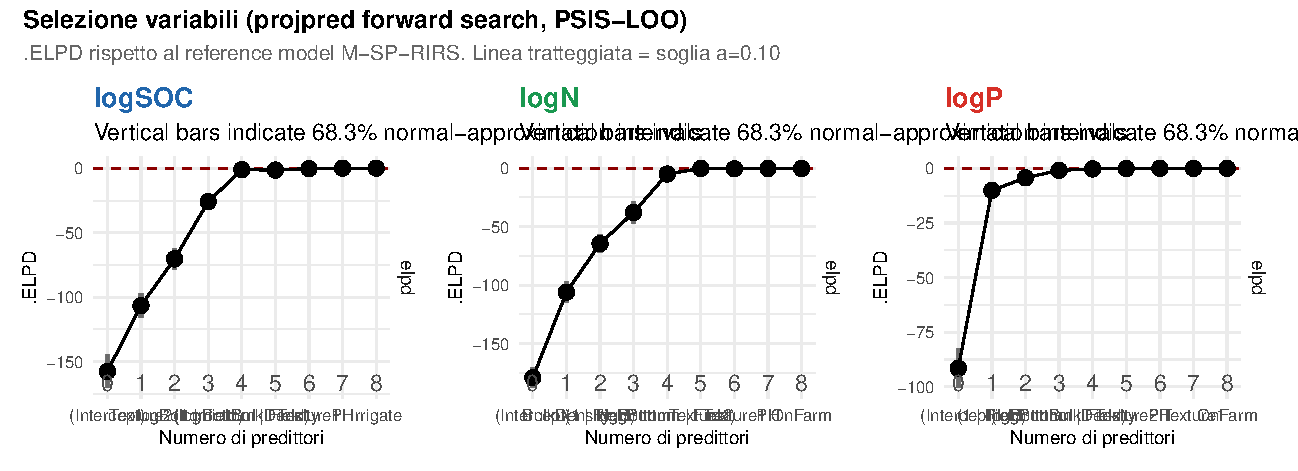
\includegraphics[width=0.95\linewidth]{fig06_projpred.pdf}
\caption{Percorso di selezione projpred per SOC, N e P ($\Delta$ELPD
in funzione del numero di predittori; linea tratteggiata:
soglia di accettazione $\alpha = 0.10$).}
\label{fig:projpred}
\end{figure}

% TESTO INTERPRETATIVO
%
% Sebbene projpred identifichi un sottoinsieme più parsimonioso di
% covariate, il modello completo è mantenuto come riferimento
% inferenziale poiché definito a priori sulla base delle ipotesi
% ecologiche considerate. Questa scelta evita procedure iterative di
% selezione guidate dai risultati osservati e riduce il rischio di
% sovrainterpretazione dei dati.

\subsection{Confronto tra strutture gerarchiche}
\label{subsec:loo}

\begin{table}[htbp]
\centering
\caption{Confronto LOO-CV tra diverse specificazioni
($\Delta$ELPD rispetto al modello multirisposta completo;
$|z| = |\Delta\text{ELPD}|/\text{SE}$).}
\label{tab:loo4}
\small
\begin{tabular}{@{}llrrr@{}}
\toprule
Modello & Descrizione & $\Delta$ELPD & SE & $|z|$ \\
\midrule

\textbf{Modello multirisposta completo}
& RE 6D cross-risposta
& $\mathbf{0.0}$
& ---
& --- \\

Modelli univariati
& RI+RS per ciascuna risposta
& $-0.4$
& $\approx 4$
& $\approx 0.1$ \\

Modello con slope proporzionale
& RI + slope proporzionale
& $-4.1$
& $4.2$
& $\approx 1.0$ \\

Modello a sole intercette casuali
& Random intercept indipendenti
& $-9.2$
& $5.7$
& $1.6$ \\

\bottomrule
\\

\end{tabular}
\end{table}

% TESTO INTERPRETATIVO
%
% Le diverse specificazioni gerarchiche mostrano prestazioni
% predittive sostanzialmente equivalenti. Il modello multirisposta
% completo è mantenuto come modello di riferimento poiché consente
% di quantificare esplicitamente le correlazioni tra nutrienti a
% livello di campo senza perdita apprezzabile di capacità predittiva.

\subsection{Analisi di robustezza}
\label{subsec:robustezza}

\subsubsection{Sensibilità alle osservazioni influenti}

Sono state identificate osservazioni con Pareto $k \geq 0.7$.
Il confronto tra modello completo e modello ridotto mostra variazioni sostanzialmente nulle nelle stime puntuali dei parametri. L'unica differenza notevole è una moderata riduzione di $\hat\sigma_r$ dopo la rimozione delle osservazioni influenti, come atteso in presenza di residui estremi. Le principali inferenze strutturali risultano robuste rispetto alla
presenza di osservazioni influenti.

\subsubsection{Sensibilità alla specificazione delle covariate}

È stato considerato un modello semplificato ottenuto rimuovendo le
covariate di \textit{management} e Texture1.

LOO:
$\Delta\text{ELPD}=+1.8$
(SE $=4.1$, $|z|=0.4$).

Il risultato conferma che management e Texture1 apportano un contributo
predittivo limitato, in accordo con l'analisi projpred.

\subsubsection{Sensibilità della struttura casuale}
CONTROLLARE STA ROBA, NON MI SEMBRA CORRETTA

È stato considerato un modello in cui N è descritto mediante una sola
intercetta casuale.

LOO:
$\Delta\text{ELPD}=-5.7$
(SE $=6.0$).

Il peggioramento predittivo è modesto ma suggerisce che la pendenza
casuale associata a N contribuisce alla descrizione della variabilità
tra campi.

\subsubsection{Verifica dell'indipendenza condizionale dei residui}

Per verificare l'ipotesi di indipendenza condizionale tra le tre risposte, il modello è stato esteso introducendo una struttura residua multivariata:

\[
\boldsymbol{\varepsilon}_{ij}
\sim
\mathcal{N}_{3}
\!\left(
\mathbf{0},
\Sigma_{\mathrm{res}}
\right).
\]

Le correlazioni residue a posteriori risultano tutte prossime allo zero:
ALLIENARE , USARE MENO SPAZIO

\[
\hat{\rho}^{\mathrm{res}}_{\mathrm{SOC}-N}
=
0.015
\ \CI{-0.121}{0.151},
\]

\[
\hat{\rho}^{\mathrm{res}}_{\mathrm{SOC}-P}
=
-0.021
\ \CI{-0.151}{0.110},
\]

\[
\hat{\rho}^{\mathrm{res}}_{N-P}
=
0.035
\ \CI{-0.096}{0.166}.
\]

La validazione predittiva mostra una lieve riduzione della capacità esplicativa:

\[
\Delta\mathrm{ELPD}
=
-3.1,
\qquad
\mathrm{SE}=1.1.
\]

Non emerge evidenza di correlazione residua aggiuntiva tra le risposte. La dipendenza tra nutrienti è quindi adeguatamente catturata dalla struttura gerarchica a livello di campo, senza necessità di una componente residua multivariata.

\subsubsection{Autocorrelazione verticale dei residui}

\paragraph{Struttura di dipendenza lungo il profilo.}

\todo{Analisi frequentista mediante \texttt{nlme} per verificare l'assenza di autocorrelazione verticale residua.}


% ==============================================================================
\section{Discussione}
\label{sec:discussione}

\subsection{SOC: correlazione slope--intercetta e meccanismi biologici}

\todo{$\hat\rho_\SOC=0.52$ [0.12, 0.80], positivo e robusto. $\tauB{\SOC}=0.22$
significativamente positivo. Campi con SOC elevato decadono pi\`u lentamente.
Confronto con letteratura (Jobbágy \& Jackson 2000;
Mutambu et al.\ 2019; Kirsten et al.\ 2019). Meccanismi possibili:
stabilizzazione organo-minerale, pratiche agronomiche. pH non significativo
($\hat\gamma_\SOC^\text{pH}=-0.02$, CI include zero).}

\subsection{N: variabilit\`a di slope senza correlazione con il livello}

\todo{$\hat\rho_N=-0.16$ con CI che include zero: le slope di N non sono correlate
ai livelli di campo. Ma $\tauB{N}=0.145$ significativamente positivo: esiste
variabilit\`a tra campi nella pendenza verticale dell'azoto, non catturata da M-SP.
Biologicamente plausibile: N mobile risponde alle pratiche pi\`u che alla struttura.}

\subsection{P: evidenza moderata}

\todo{$\hat\rho_P = 0.478$ con CI\,90\% ampio $[-0.29, 0.88]$: evidenza moderata
ma alta incertezza. $\tauB{P} = 0.094$ borderline (CI\,90\% $[0.007, 0.189]$).
Cautela nell'interpretazione: il pattern esiste ma non \`e robusto.}

\subsection{Effetti di management e pH}

\todo{$\hat\beta_r$ deboli (CI\,90\% quasi sempre su zero per la maggior parte).
pH non significativo per nessuna risposta ($\hat\gamma^\text{pH} \approx 0$).
Projpred: n\`e pH n\`e management entrano nei modelli selezionati per nessuna
risposta. La variabilit\`a tra campi \`e catturata dalla struttura bivariata
RI+RS pi\`u che dalle pratiche osservate.}

\subsection{Indipendenza condizionale tra nutrienti e legame SOC--N}

I tre nutrienti risultano condizionalmente indipendenti dati i
predittori di M-SP-RIRS-MVRE: le correlazioni residue (M-SP-RIRS-MV) sono $\approx 0$
e aggiungere tale struttura non migliora il LOO.
La co-variazione osservata tra SOC, N e P \`e interamente catturata da
profondit\`a, tessitura e struttura di campo.
Il legame SOC--N emerge per\`o a livello di effetti casuali di campo nel modello finale:
$\hat\rho^{\mathrm{int}}_{\SOC\text{-}N} = +0.386\ [0.038, 0.667]$ (CI\,90\% lontano da zero).
Questo segnale biologicamente interpretabile — i campi pi\`u fertili in SOC tendono
ad essere pi\`u fertili in N, al di l\`a dei predittori osservati — costituisce il
risultato principale aggiunto dal modello M-SP-RIRS-MVRE rispetto a M-SP-RIRS.


% ==============================================================================
\section{Conclusioni}
\label{sec:conclusioni}

\todo{(1) SOC: $\hat\rho_\SOC=0.52$ [0.12, 0.80], robusto. I campi con SOC
elevato decadono pi\`u lentamente in profondit\`a.
(2) N: $\hat\rho_N\approx -0.16$ (CI su zero), ma $\tauB{N}=0.145$ positivo:
la variabilit\`a di slope esiste ma non \`e correlata al livello medio.
(3) P: $\hat\rho_P=0.48$ con alta incertezza.
(4) pH non aggiunge potere predittivo in questo dataset.
(5) Nuovo in MVRE: $\hat\rho^{\mathrm{int}}_{\SOC\text{-}N}=+0.386$ [0.038, 0.667]:
legame biologico SOC--N identificabile a livello di campo, al di l\`a dei predittori osservati.
Dal punto di vista metodologico: M-SP-RIRS-MVRE generalizza M-SP-RIRS
stimando congiuntamente gli effetti di campo delle tre risposte.
Implicazioni pratiche per la gestione del suolo in Tanzania.}


% ==============================================================================
\bibliography{refs}


% ==============================================================================
\appendix

\section{Trace plot e posterior predictive check}
\label{app:trace}

\begin{figure}[htbp]
  \centering
  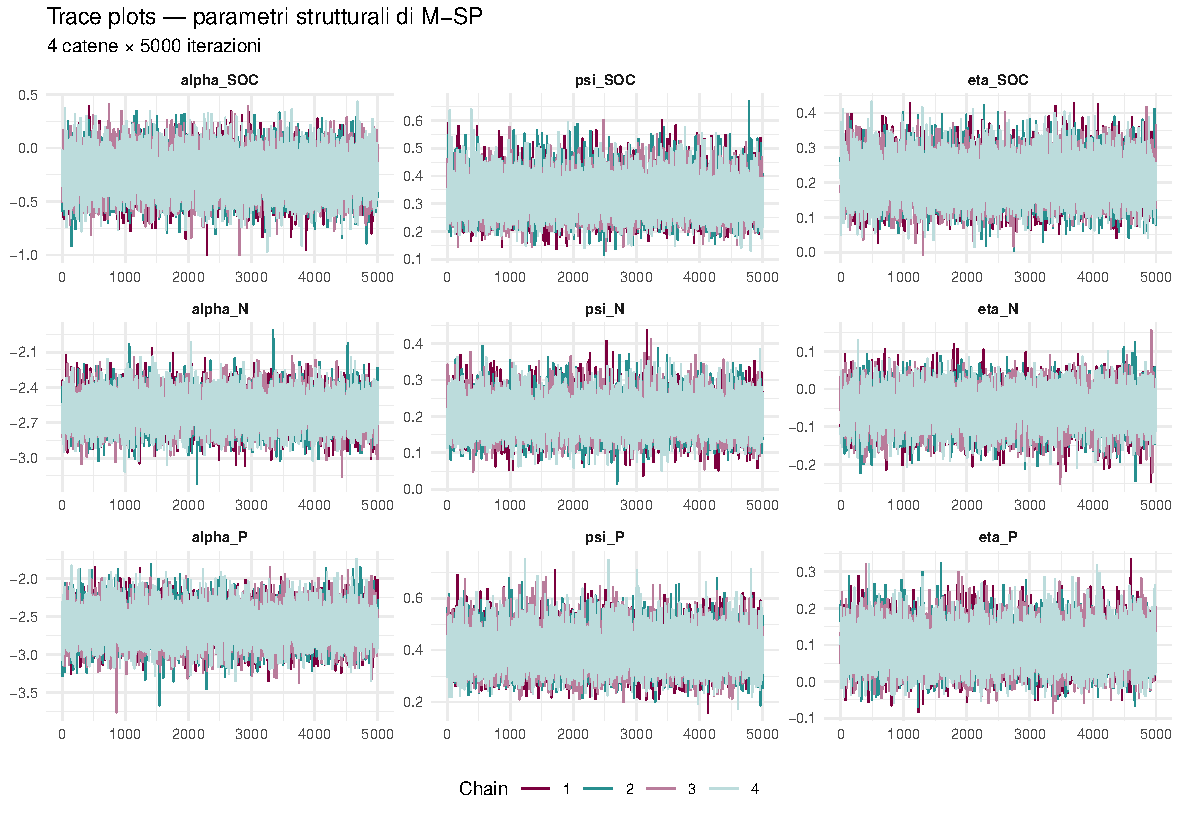
\includegraphics[width=0.8\linewidth]{appfig02_trace.pdf}
  \caption{Trace plot delle 4 catene MCMC per $\alpha_r$, $\tauA{r}$, $\tauB{r}$, $\rho_r$
    (modello M-SP-RIRS-MVRE). Buona mescolanza: nessuna evidenza di mancata convergenza.}
  \label{fig:trace}
\end{figure}

\end{document}
